\chapter{The JUNO detector}
The Jiangmen Underground Neutrino Observatory~(JUNO) is a multi-functional neutrino experiment project in southern China, as shown in Fig.~\ref{fig:juno_site}. The Central Detector~(CD) is located in a laboratory \SI{700}{m} underground~\cite{muon207}. Its excellent energy resolution and relatively large effective volume provide an exciting opportunity to address many important issues in the fields of neutrino and astroparticle physics. As evidenced in Tab.~\ref{tab:juno_core}, there are two nuclear power plants, Yangjiang~(YJ) and Taishan~(TS), at around \SI{53}{km} away from the JUNO detector. After 2000 days of data taking, the measurement result of NMO can be obtained with a confidence level of $3\sigma$.

\begin{figure}[htbp]
	\centering
	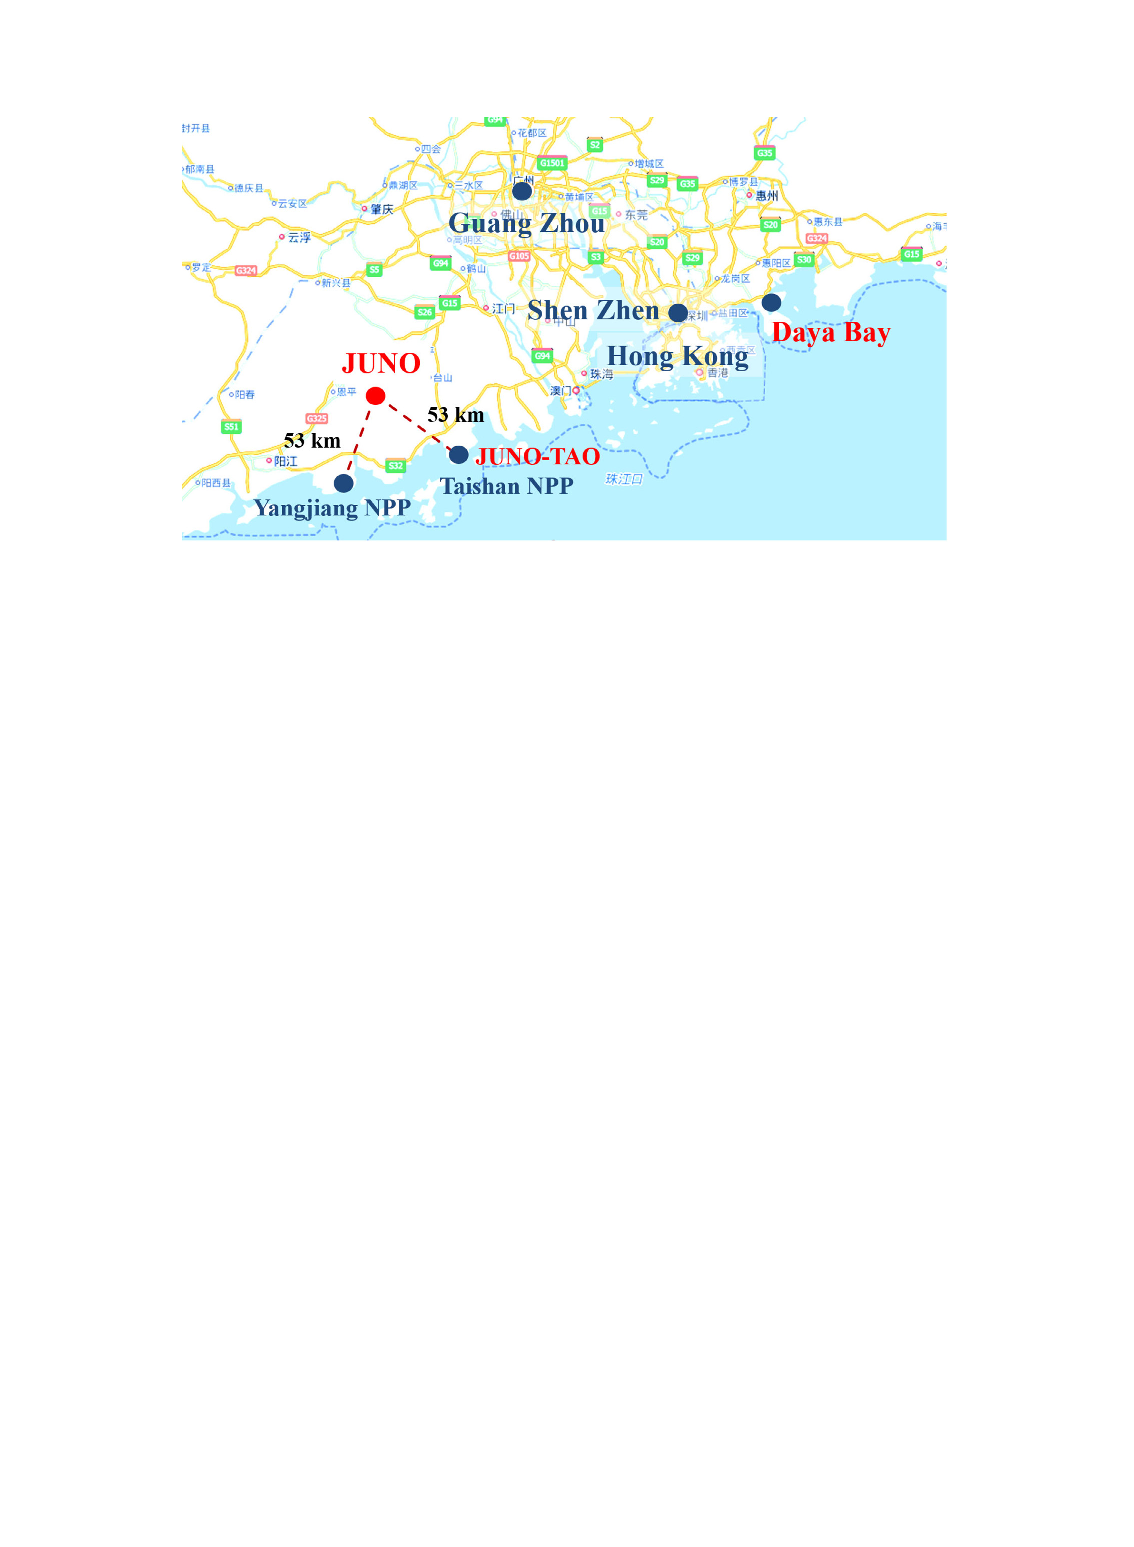
\includegraphics[width=0.7\textwidth]{junoDetector/location.pdf}
	\caption{The location of JUNO~\cite{muon207}: Jinji, Kaiping city, Jiangmen city, Guangdong province, China. Its geographical location is $112^{\circ}31^{\prime}05^{\prime\prime}~\mathrm{E}$ and $22^{\circ}07^{\prime}05^{\prime\prime}~\mathrm{N}$.}
	\label{fig:juno_site}
\end{figure}

\begin{table}[htbp]
	\centering % 表格居中
	\caption{The power of the reactor core and the baseline distance, the data comes from~\cite{juno_yellow_book}}
	\label{tab:juno_core}
	\begin{tabular}{cccccccc}
		\toprule % 顶线
		\textbf{Cores}     & YJ-C1 & YJ-C2 & YJ-C3 & YJ-C4 & YJ-C5 & YJ-C6 \\
		\midrule
		Power~(\si{GW})    & 2.9   & 2.9   & 2.9   & 2.9   & 2.9   & 2.9   \\
		Baseline~(\si{km}) & 52.75 & 52.84 & 52.42 & 52.51 & 52.12 & 52.21 \\
		\addlinespace
		\textbf{Cores}     & TS-C1 & TS-C2 & TS-C3 & TS-C4 & DYB   & HZ    \\
		\midrule
		Power~(\si{GW})    & 4.6   & 4.6   & 4.6   & 4.6   & 17.4  & 17.4  \\
		Baseline~(\si{km}) & 52.76 & 52.63 & 52.32 & 52.20 & 215   & 265   \\
		\bottomrule
	\end{tabular}
\end{table}

% \begin{figure}[htbp]
% 	\centering
% 	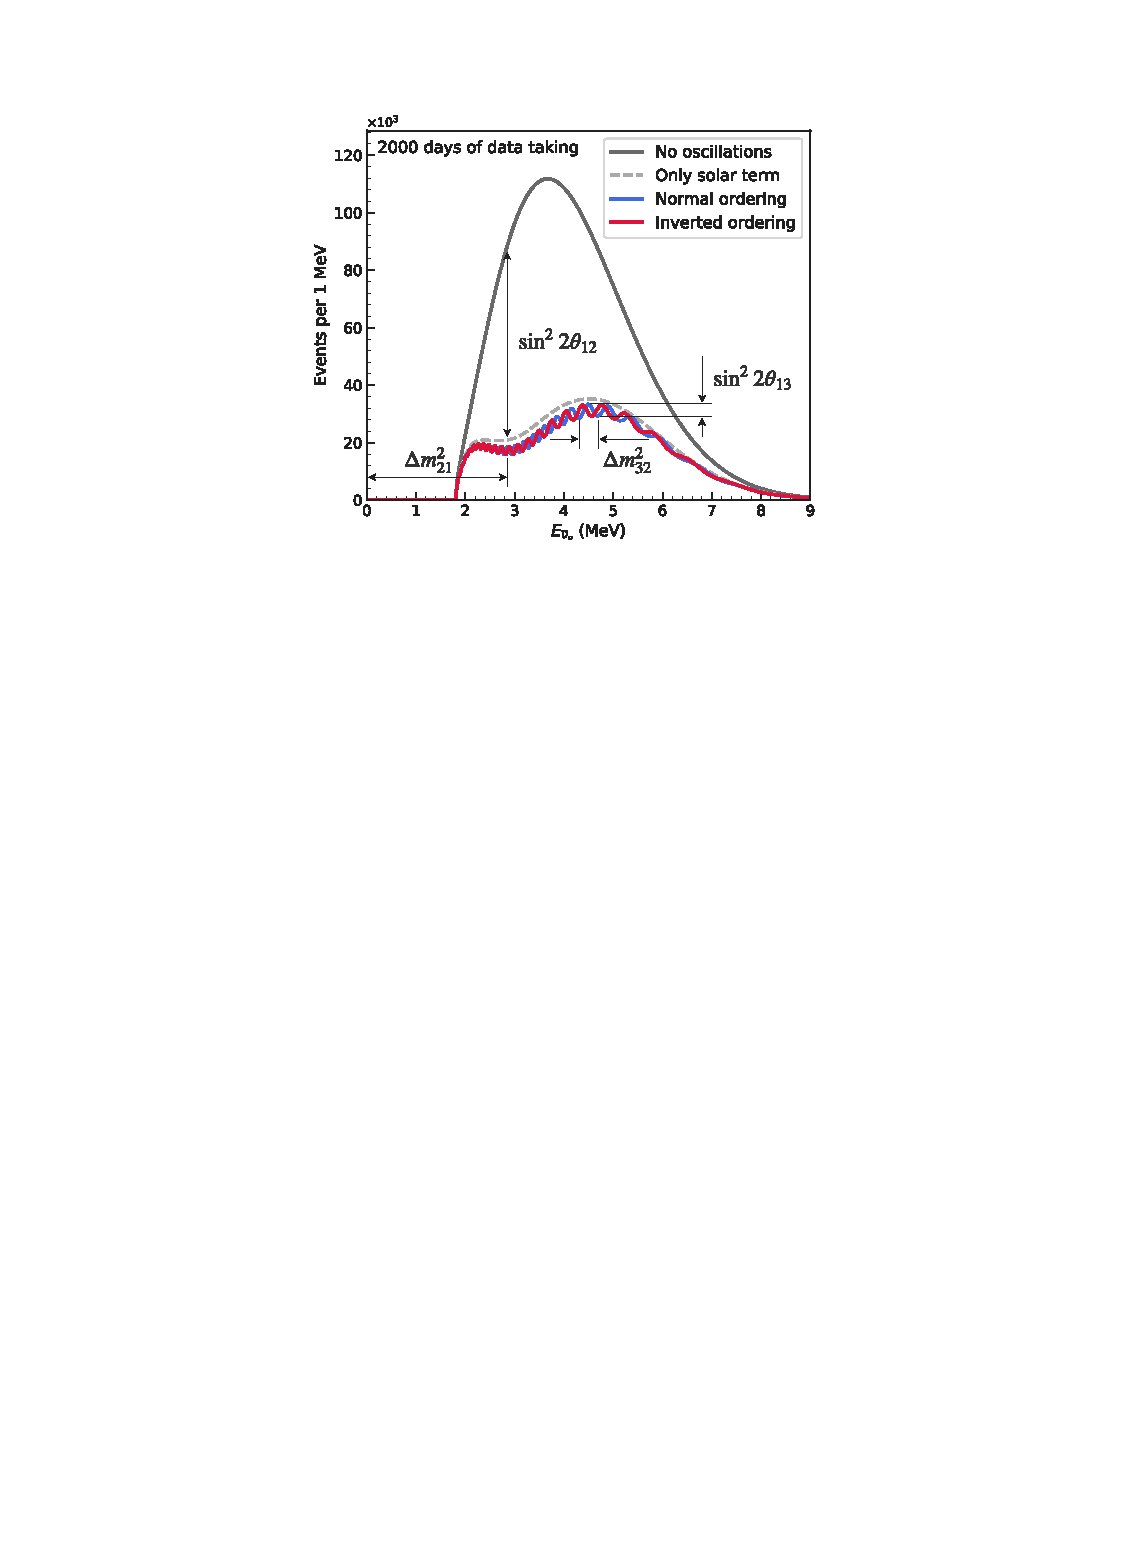
\includegraphics[width=0.5\textwidth]{junoDetector/nmo_2000day.pdf}
% 	\caption{The sensitivity of NMO measurement at JUNO after 2000 days of data taking based on simulation. Four oscillation parameters are depeended on~\cite{muon207}.}
% 	\label{fig:juno_nmo_2000}
% \end{figure}

\section{The design of JUNO Central Detector}
\label{sec:juno_cd_design}
The JUNO detector is composed of CD, a water Cherenkov detector based on the water pool~(WCD), and a Top Tracker~(TT), as illustrated in Fig.~\ref{fig:juno_cd_structure}.
\begin{figure}[htbp]
	\centering
	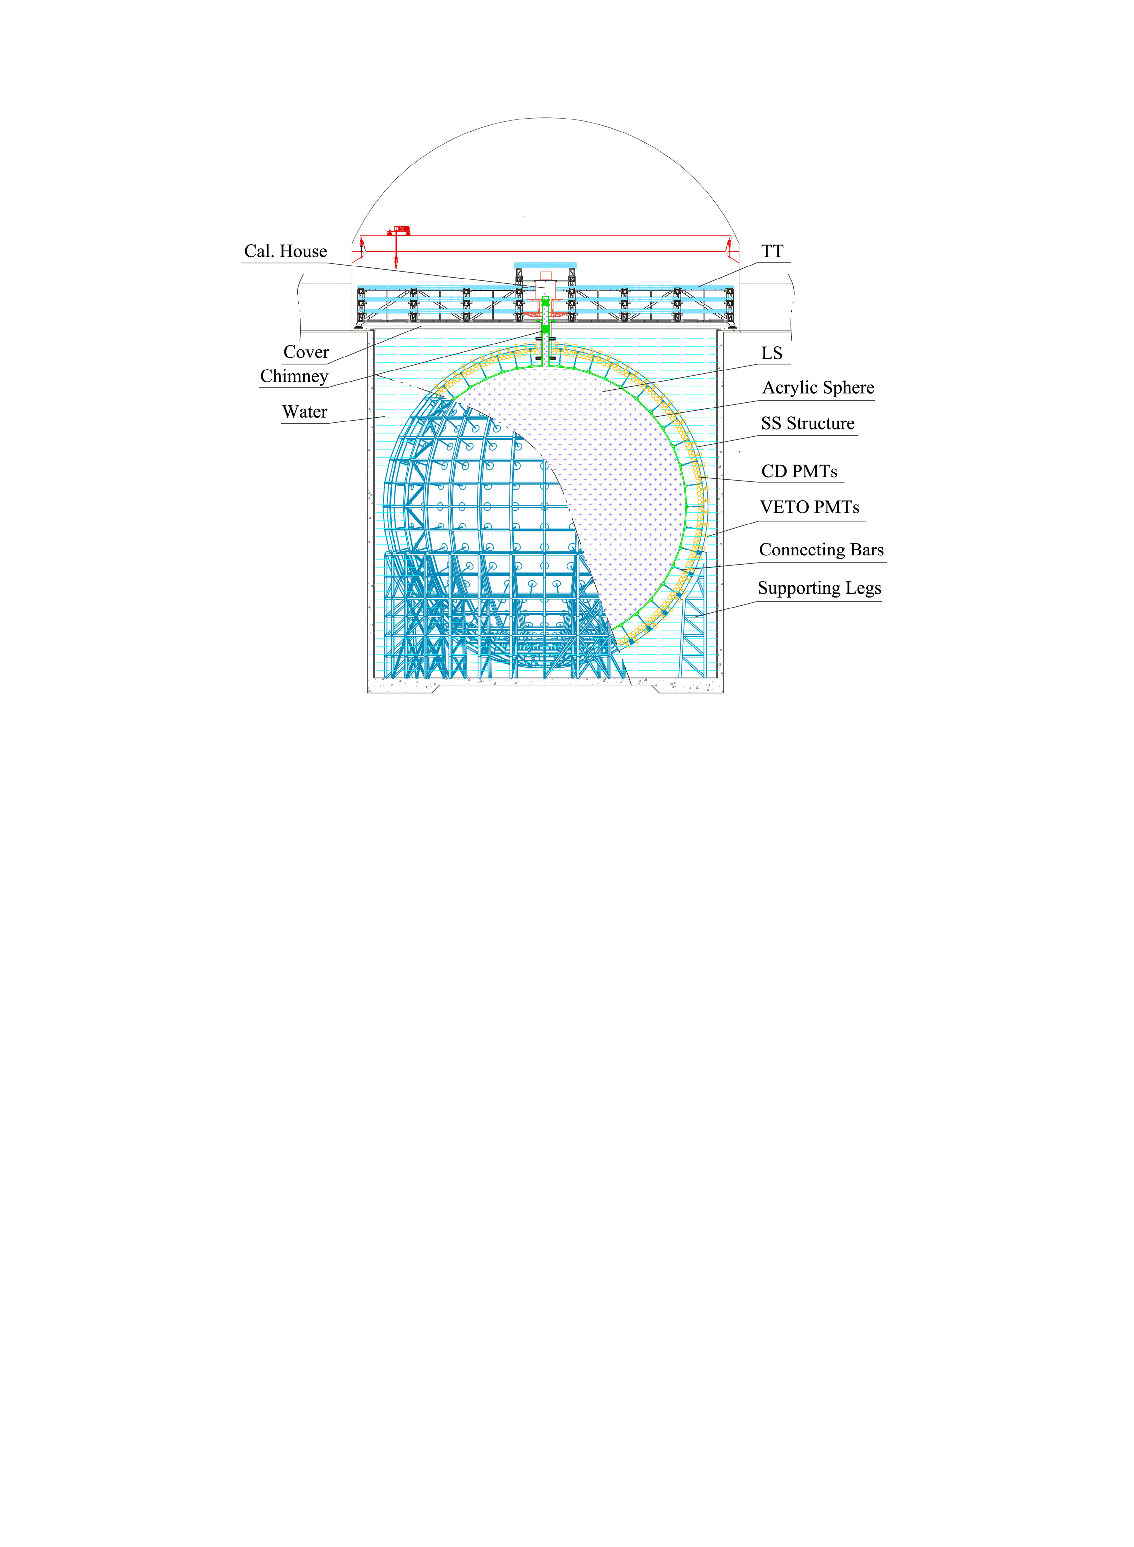
\includegraphics[width=0.6\textwidth]{junoDetector/structure.pdf}
	\caption{The structure of JUNO detector. The figure comes from~\cite{muon207}}
	\label{fig:juno_cd_structure}
\end{figure}
\subsection{The structure of Central Detector}
The Central Detector consists of an acrylic spherical shell with a diameter of \SI{35.4}{m} and a thickness of \SI{12}{cm}, which is filled with \SI{20}{kton} of liquid scintillator~\cite{JUNO_CD_tech}. It is engineered to attain an energy resolution of $\frac{\SI{3}{\%}}{\sqrt{E}}$ to facilitate the measurement of NMO. To detect the photons emitted due to the energy deposited by particles, 17,612 20-inch and 25,600 3-inch photomultiplier tubes~(PMTs), more detailed information in Tab.~\ref{tab:juno_pmt}, are mounted on a spherical structure with a radius of \SI{19.5}{m}. This setup achieves a photocathode coverage rate of over \SI{75}{\%}. Ultra-pure water is filled between the PMT and the acrylic to shield the radioactive background from the surface of the PMT. The entire CD detector is immersed in a cylindrical water pool to shield the radioactive background from the surrounding rocks, etc. At the same time, the water pool, as a Cherenkov detector, is equipped with 1,600 20-inch PMTs, enabling the detection of \SI{99.8}{\%} of cosmic muons. To avoid the interference of the geomagnetic field, a set of 32 circular coils surrounding the detector is designed to keep the residual magnetic field in the PMT area of CD less than \SI{0.05}{G} and that in WCD below \SI{0.1}{G}~\cite{muon207}.

\begin{table}[htbp]
	\centering % 表格居中
	\caption{The summary of PMTs used in JUNO CD, the data comes from~\cite{muon207,PMT-3inch,JUNO:2022hlz}}
	\label{tab:juno_pmt}
	\begin{tabular}{cccccccc}
		\toprule % 顶线
		    & Size~(\si{inch}) & Type       & Number & Manufacturer                               \\
		\midrule % 中线
		CD  & 20               & MCP-PMT    & 12612  & Northern Night Vision Technology Co.       \\
		    &                  & Dynode-PMT & 5000   & Hamamatsu Photonics K. K.                  \\
		    & 3                & SPMT       & 25600  & Hainan Zhanchuang Photonics Technology Co. \\
		WCD & 20               & MCP-PMT    & 2400   & Northern Night Vision Technology Co.       \\
		\bottomrule % 底线
	\end{tabular}
\end{table}

\subsection{The Top Tracker}
It is mainly used to reconstruct and track the trajectories of atmospheric muons. This detector is modified from the target tracker modules of the decommissioned OPERA experiment. It covers approximately \SI{60}{\%} of the area at the top of CD and contains 63 double-layer scintillator walls~(a total of 496 modules), as shown in Fig.~\ref{fig:TT_0}. Each module is composed of plastic scintillator strips arranged orthogonally, and the signals are read out through wavelength-shifting fibers connected to multi-anode PMTs~(MA-PMTs), as illustrated in Fig.~\ref{fig:juno_TT}. To adapt to the highly radioactive environment of the underground laboratory, its electronics system has been comprehensively upgraded to achieve precise triggering at high counting rates. TT can significantly reduce the interference of cosmic muon spallation background on the measurement of NMO through the reconstruction of muon trajectories with centimeter-level accuracy. It is particularly crucial for identifying the \ce{^9Li}/\ce{^8He} background induced by muons~\cite{top_tracker,muon207}.

\begin{figure}[htbp]
	\centering
	\begin{subfigure}{0.75\textwidth}
		\centering
		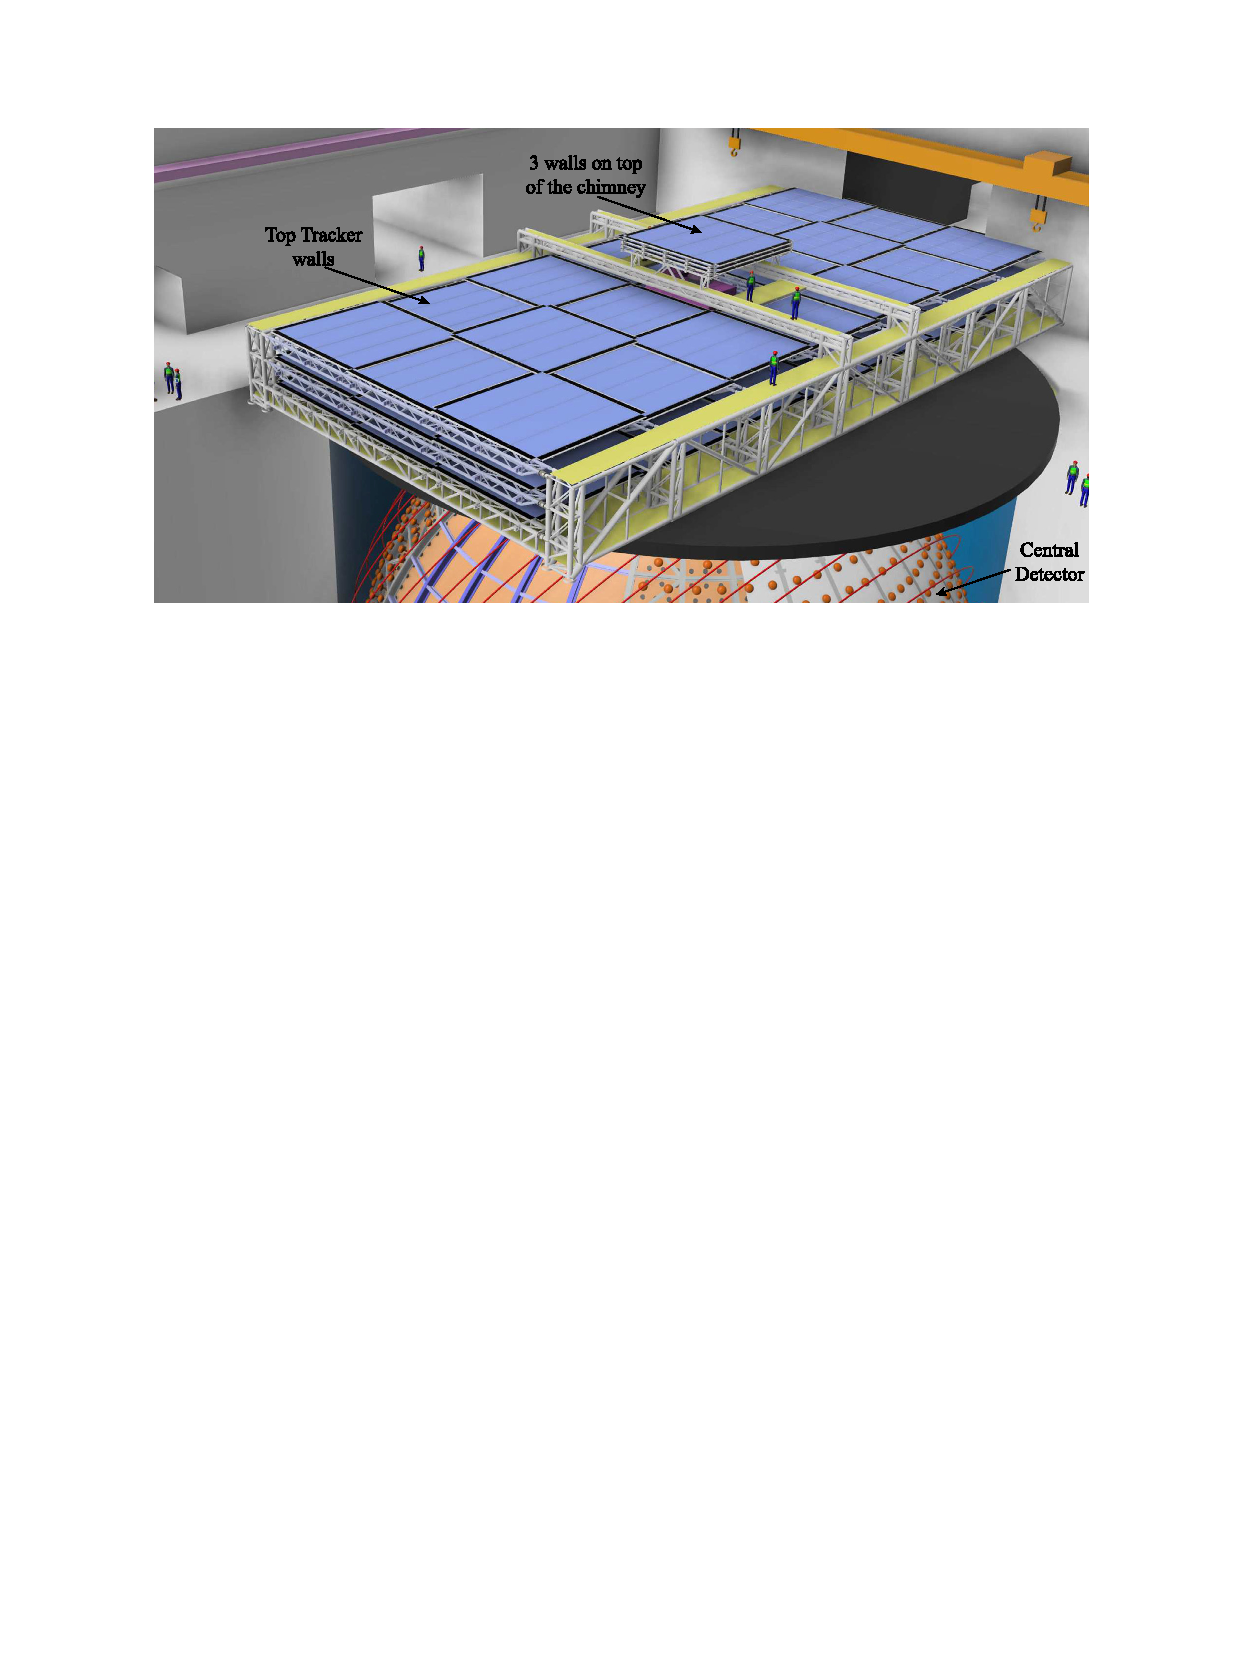
\includegraphics[width=\textwidth]{junoDetector/TT_0.pdf}
		\caption{}
		\label{fig:TT_0}
	\end{subfigure}%
	\hfill
	\begin{subfigure}{0.5\textwidth}
		\centering
		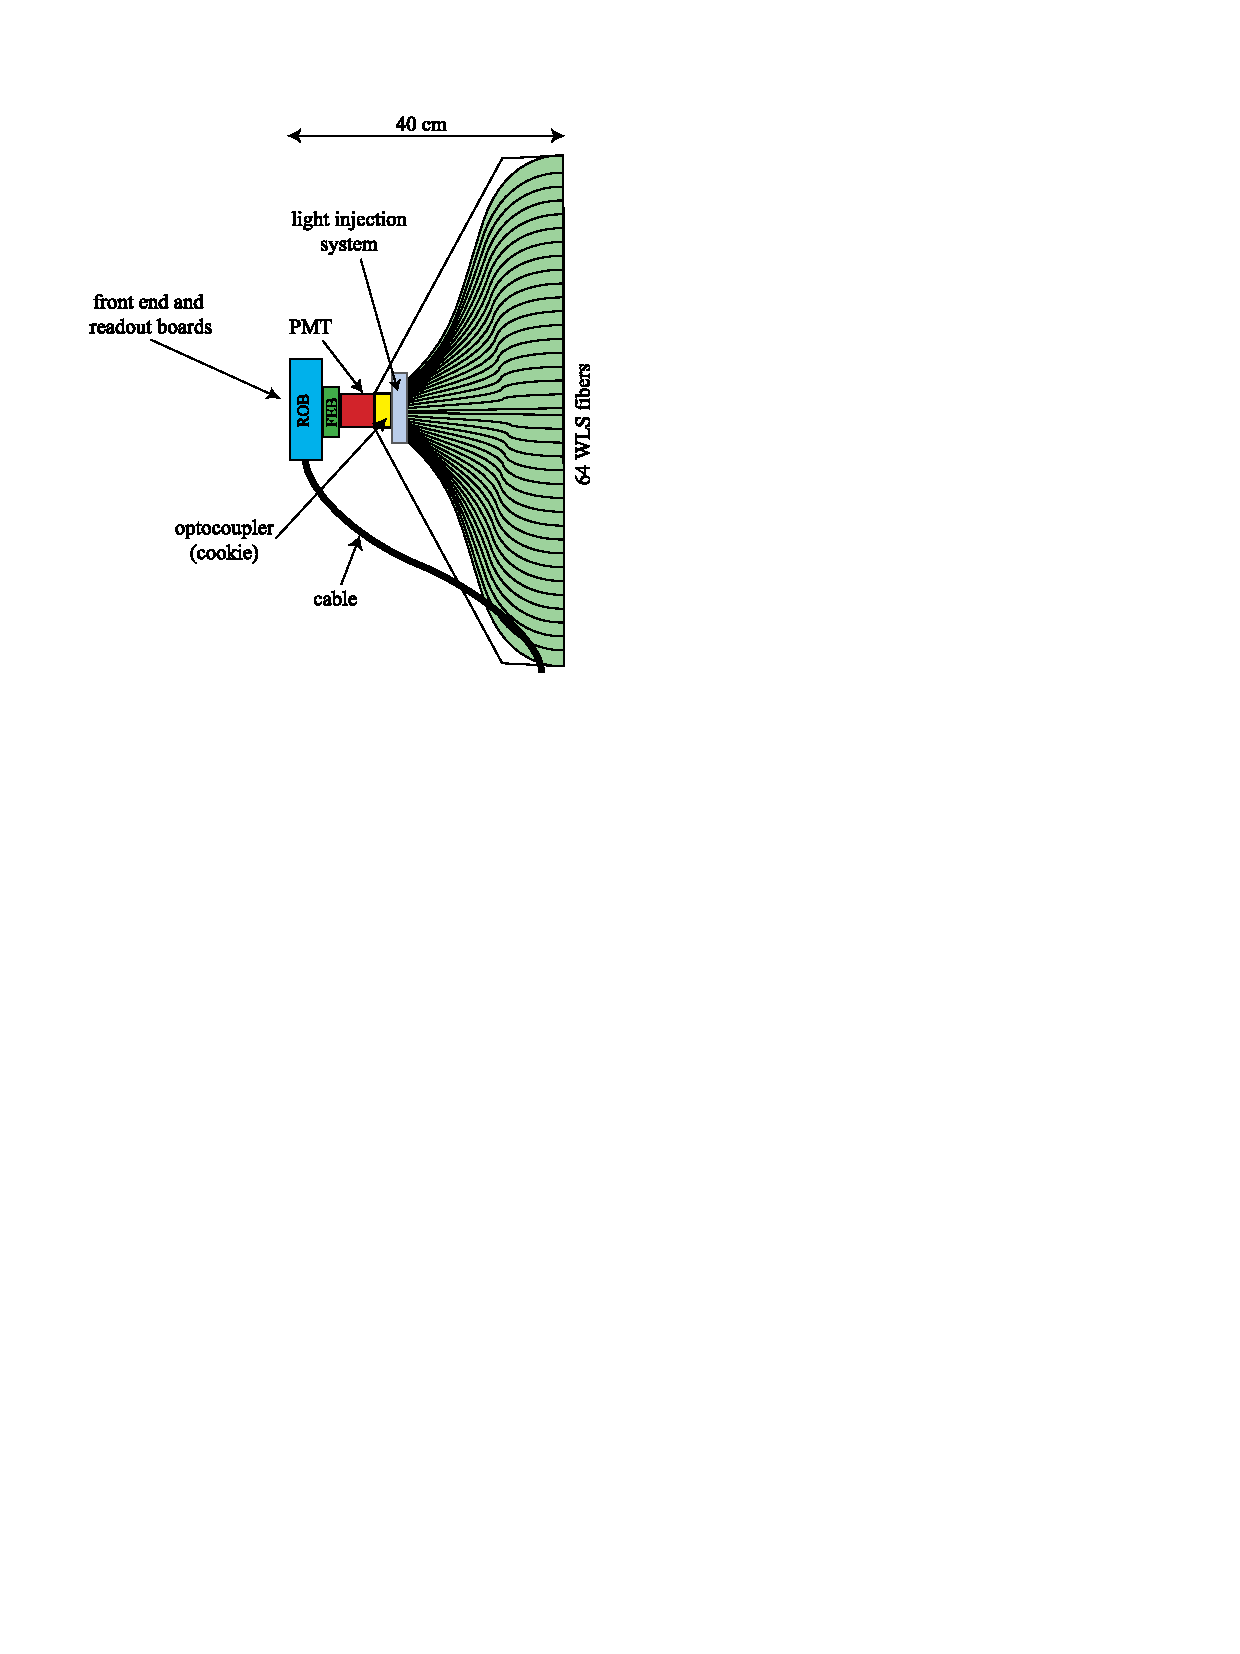
\includegraphics[height=6cm]{junoDetector/TT_1.pdf}
		\caption{}
		\label{fig:TT_1}
	\end{subfigure}%
	\hfill
	\begin{subfigure}{0.5\textwidth}
		\centering
		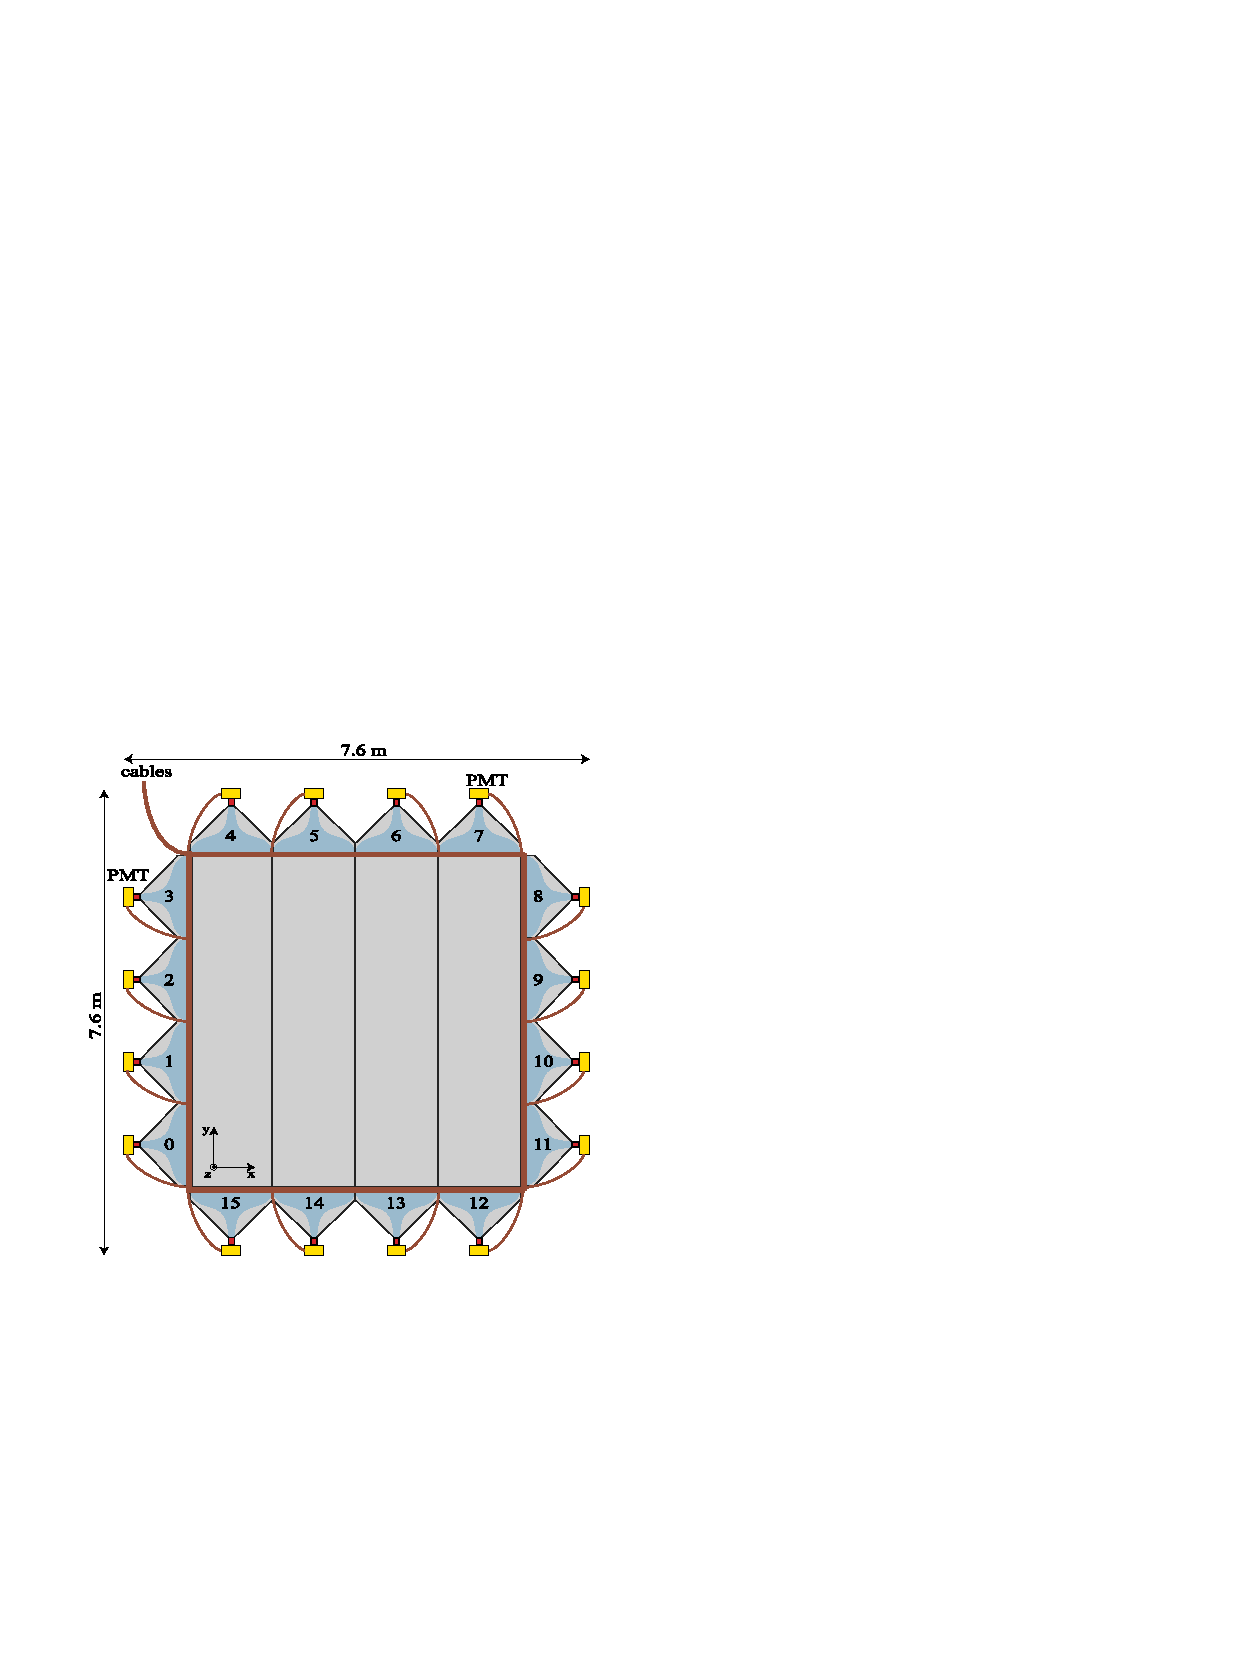
\includegraphics[height=6cm]{junoDetector/TT_2.pdf}
		\caption{}
		\label{fig:TT_2}
	\end{subfigure}
	\caption{\subref{fig:TT_0} presents the side view of TT from the CD side. \subref{fig:TT_1} is a schematic illustration of a TT module. This module is composed of 64 strips that are read out by WLS fibers and \subref{fig:TT_2} depicts a plastic scintillator strip wall. These figures are sourced from~\cite{top_tracker}.}
	\label{fig:juno_TT}
\end{figure}

\section{The trigger system of JUNO CD}
\label{sec:juno_trigger}
\subsection{The Multi-Messenger Trigger}
To efficiently and accurately select the physics events of interest from the large volume of detector data, the JUNO experiment has implemented several trigger systems. As a crucial component of the data acquisition chain, the trigger system directly impacts event recording efficiency, data quality, and the effectiveness of subsequent physics analyses. The Multi-Messenger~(MM) trigger~\cite{MMtrigger} is designed to enable the detection of low-energy events that are relevant to both neutrino and astrophysical physics.
In contrast to the multiplicity-based Global Trigger, which mainly depends on the number of detected photons within a single time window to initiate an event readout, MM Trigger is based on a number of likelihood and machine-learning, using the PMT timing and position information. It enables the detection of low-energy events that are relevant to both neutrino and astrophysical physics, and optimizes the discrimination between physics events and dark noise induced events to reduce the data volume.
\subsection{The Multiplicity Software Trigger}

\section{The calibration system in JUNO}
\label{sec:juno_calibration}
\subsection{The laser calibration}
\subsection{The position and uniformity calibration}
\subsection{The energy calibration}

\section{The Simulation Software of JUNO CD}
\label{sec:juno_simulation}
\section{The subdetector of JUNO}
\label{sec:juno_subdetector}
In the measurement of NMO, two extremely crucial factors are the input reactor neutrino energy spectrum and the purity of LS. JUNO has designed a sub-detector TAO at Taishan to provide an accurate input energy spectrum. During the liquid scintillator filling period, in order to detect the background content of LS, the OSIRIS detector has been designed and operated beside the JUNO CD.

\subsection{The Taishan Antineutrino Observatory}
The Taishan Antineutrino Observatory~(TAO) serves as a satellite detector of JUNO. It is positioned \SI{30}{m} away from the reactor core of the Taishan Nuclear Power Plant. The core of TAO consists of a spherical acrylic vessel with a diameter of \SI{1.8}{m}, which is filled with \SI{2.8}{m^3} of gadolinium-doped liquid scintillator~(Gd-LS)~\cite{TAO_wangzhimin}, as shown in Fig.~\ref{fig:tau_structure}. This detector innovatively employs a \SI{10}{m^2} silicon photomultiplier~(SiPM) array to fully cover the spherical vessel. When combined with the \SI{-50}{\degreeCelsius} cryogenic operation technology, the dark noise is significantly reduced, achieving an ultra-high collection efficiency of \SI{4500}{PE/MeV}. After an effective volume with a radius of \SI{1.3}{m}, a revolutionary energy resolution of $2\%/\sqrt{E}$ is realized~\cite{TAO_wangzhimin}. Combined with high statistics, TAO will measure the reactor neutrino energy spectrum more accurately and with lower uncertainty than CD, as illustrated in Fig.~\ref{fig:tau_uncertainty}. It will provide an important reference energy spectrum for JUNO to determine NMO~\cite{Tao_design}. At the same time, TAO can also verify nuclear databases and explore applications in reactor monitoring.
\begin{figure}[htbp]
	\centering
	\begin{subfigure}{0.5\textwidth}
		\centering
		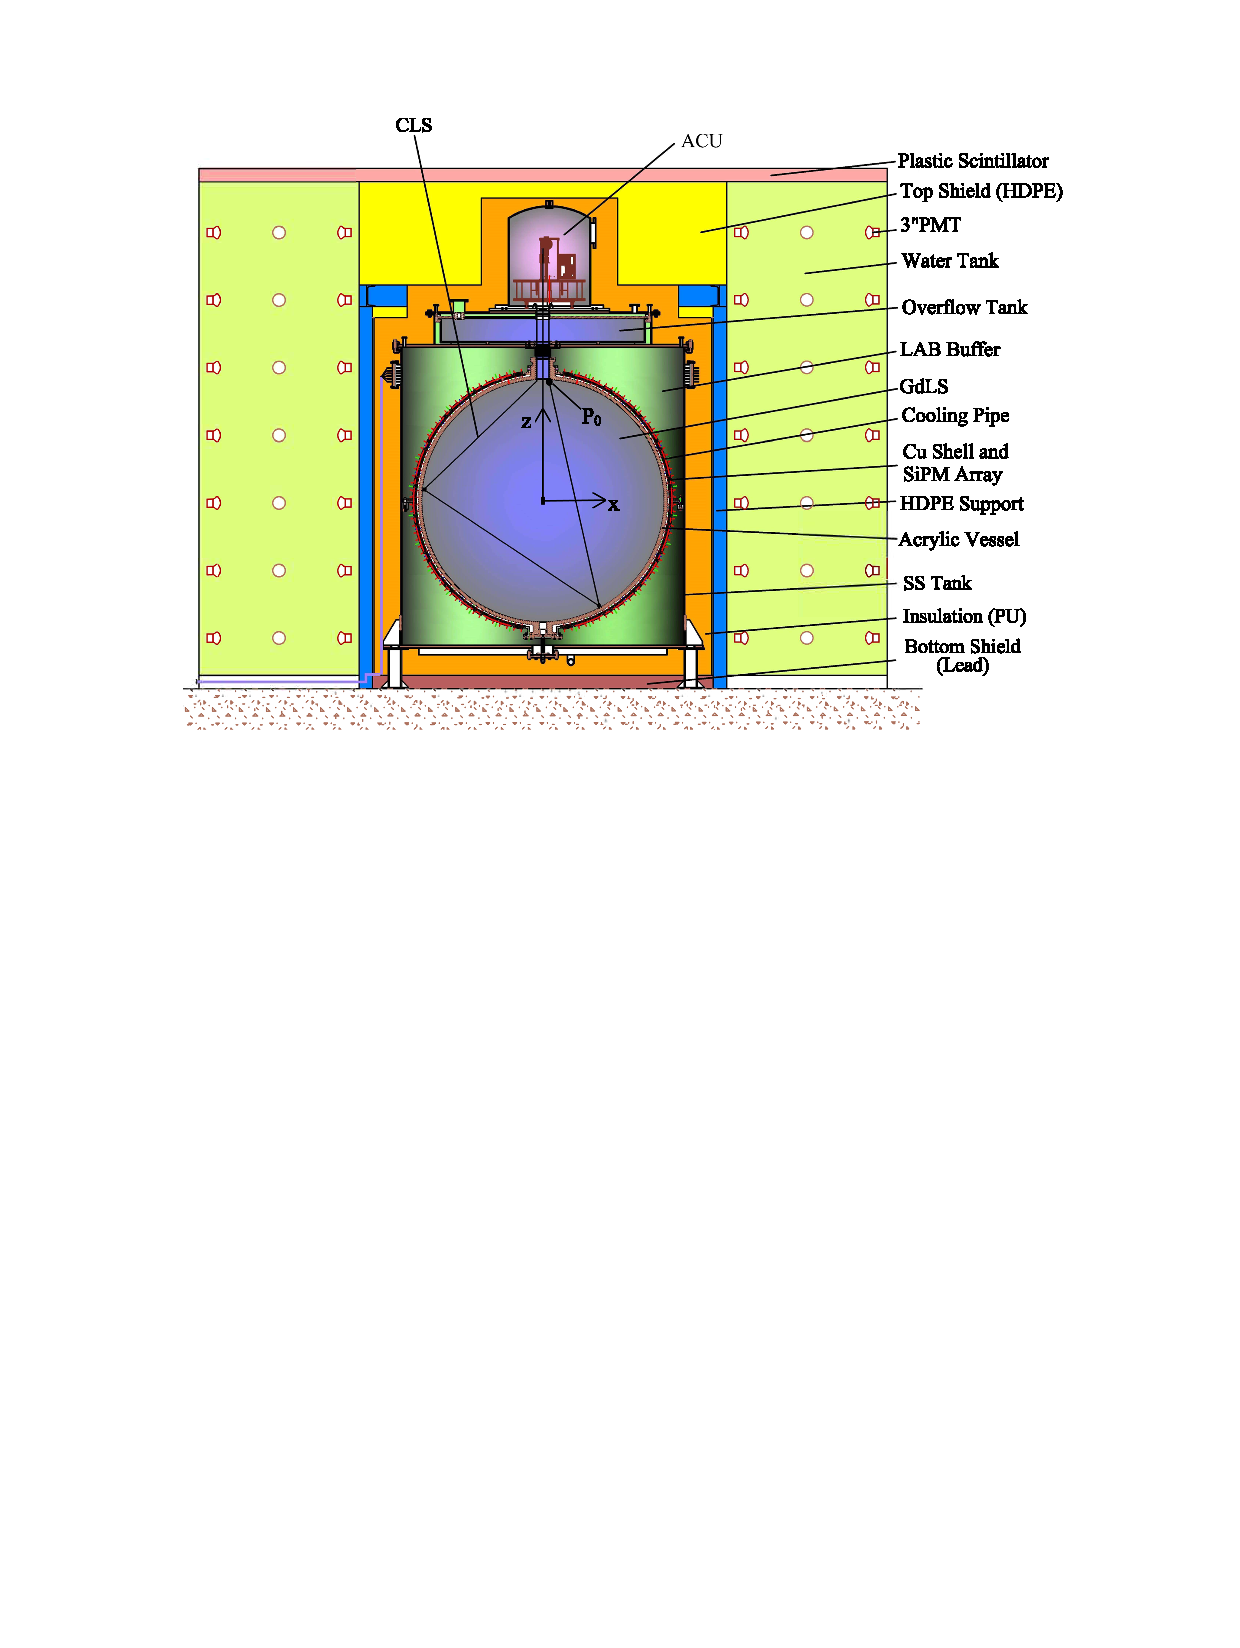
\includegraphics[height=5cm]{junoDetector/TAO_structure.pdf}
		\caption{}
		\label{fig:tau_structure}
	\end{subfigure}%
	\hfill
	\begin{subfigure}{0.5\textwidth}
		\centering
		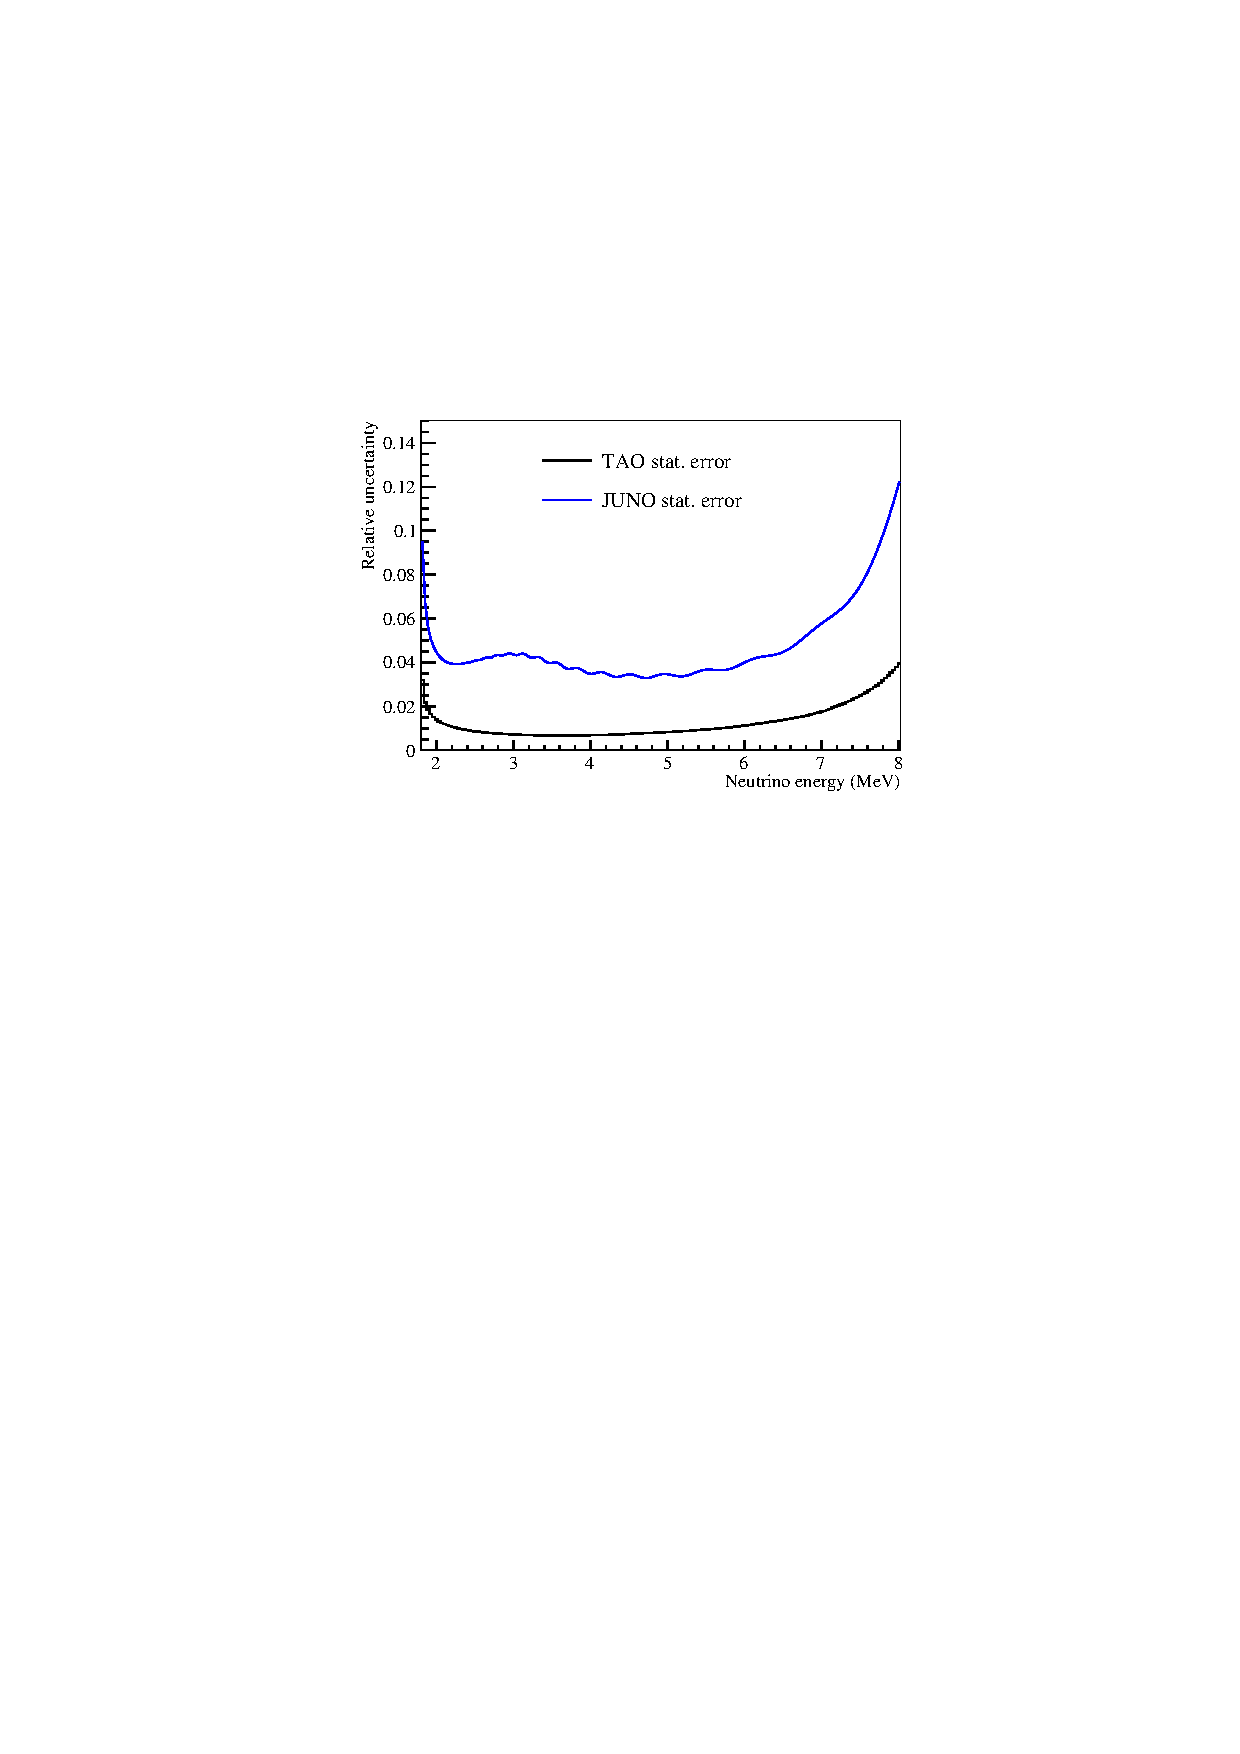
\includegraphics[height=4.5cm]{junoDetector/TAO_uncertainty.pdf}
		\caption{}
		\label{fig:tau_uncertainty}
	\end{subfigure}
	\caption{\subref{fig:tau_structure} presents the structure of TAO, this figure comes from~\cite{TAO_calib}. \subref{fig:tau_uncertainty} is showing the uncertainty of energy spectrum at JUNO CD and TAO, this figure comes from~\cite{Tao_design}.}
	\label{fig:juno_tao}
\end{figure}
\subsection{The Online Scintillator Internal Radioactivity Investigation System}
The Online Scintillator Internal Radioactivity Investigation System~(OSIRIS)
\section{The JUNO detector during water phase}
\label{sec:juno_water}